\documentclass[man]{apa2}

\usepackage{pslatex}
\usepackage{pdfsync}
\usepackage{amssymb}
\usepackage{graphicx}
\usepackage{color}
%\usepackage{apacite2}
% \usepackage{amsmath}
% \usepackage{topcapt}
\usepackage{setspace}
%\singlespacing
\usepackage{appendix}


\title{The role of context in young children's comprehension of negation}
\author{Ann E. Nordmeyer and Michael C. Frank}
\affiliation{Department of Psychology, Stanford University}

\shorttitle{Context and negation}


\abstract{Negation is an important concept in human language, yet little is known about children's ability to comprehend negative sentences. In this paper, we explore how 2--5-year-old children's comprehension of negation changes depending on the context in which a negative sentence occurs.  We collected eye-tracking data while children watched a video in which they heard positive and negative sentences. Negative sentences, such as ``look at the boy with no apples,'' referred to a boy with nothing (Experiment 1) or a boy with an alternative object (Experiment 2).   All children showed greater difficulty in resolving the referent when negative sentences referred to the boy with nothing, despite suggestions that nonexistence negations of this type are produced early in development. In addition, 3- and 4-year-old children showed an initial tendency to look away from the target and towards the named noun when the referent of the negative utterance was an alternative object.  We argue that the processing of negation in young children is influenced by the cognitive demands of the pragmatic context in which the negative utterance occurs.\\
\vspace{1cm}
Keywords: negation; language development; pragmatics}

\acknowledgements{Thanks especially to the staff and families at the San Jose Children's Discovery Museum. This work was supported by an NSF Graduate Research Fellowship to AEN and a John Merck Scholars Fellowship to MCF. An earlier version of this work was presented to the Cognitive Science Society in \citeA{nordmeyer2013}.

~\\

\noindent Address all correspondence to Ann E. Nordmeyer, Stanford University, Department of Psychology, Jordan Hall, 450 Serra Mall (Bldg. 420), Stanford, CA, 94305. Phone: 650-721-9270. E-mail: \texttt{anordmey@stanford.edu}}


\begin{document}
\maketitle

%%%%%%%%% INTRO %%%%%%%%% 
\section{Introduction}

``No'' is among the first words that children learn, as well as one of the most important.  Negation is a fundamental element of human language---it is essential to logical systems, allows us to evaluate whether a statement is true or false, and it gives us a way to express concepts such as nonexistence.  But negation can be challenging even for adult language users, who take longer to process negative sentences than positive ones \cite<e.g.>{hclark1972}.  These findings lead to an apparent paradox: How is it that negation is difficult for adults, yet acquired at such a young age?  One possibility is that many studies of negative sentence processing violate the pragmatics of negation; when negative sentences are presented in supportive contexts, the processing difficulties of negation are diminished \cite<e.g.>{wason1965}.  The goal of our current study is to explore the role that context plays in children's processing of negative sentences. We begin by reviewing research on the acquisition of negation.

\subsection{The acquisition of negation}

Negative words and morphemes like ``no,'' ``not,'' and ``-n't'' allow speakers to express multiple, related ideas.  Three primary categories have been identified in children's early negative utterances: \emph{nonexistence}, \emph{refusal}, and \emph{denial/truth-functional} negation \cite{bloom1970, bloom1993, pea1980}.  A child expressing \emph{refusal} might say ``no go outside'' when she wants to stay inside, while a child who says ``no more juice'' to describe an empty cup is expressing \emph{nonexistence} \cite{bloom1970}.  \emph{Denial} involves making a statement about falsehood; a child might say ``that not lollipop'' if she believes a candy has been falsely identified as a lollipop.  Some authors identify additional types of negation as well: \emph{self-prohibition}, expressed when the child is about to engage in a forbidden action, and \emph{unfulfilled expectations}, used when an expected action/object is not present \cite{pea1980}.  One taxonomy identified a full 9 categories of negation, including \emph{failure, inability, epistemic negation} (e.g. ``I don't know''), and \emph{inferential negation} (i.e. negation of inferred beliefs of others; \citeNP{choi1988}).  Although these different taxonomies categorize negative utterances in different ways, they all recognize that negation is used in varied contexts to express a wide range of meanings.

The acquisition of these different types of negation follows a long developmental trajectory. As early as 12 months, children produce negation in the form of the word ``no,'' typically to express nonexistence and refusal \cite{bloom1970, bloom1993, pea1980}.  Yet more complex denial negation often does not emerge until just before the second birthday  \cite{pea1980}.  Cross-linguistic studies suggest that this stratification by type---with certain negative categories produced earlier than others---can be seen across languages \cite{mcneill1968}.  
Even after age 2, children continue to learn about negation, showing changes in the syntactic forms they use to produce these ideas \cite{klima1966, cameron2007} and increases in the frequency with which they produce negatives spontaneously \cite{pea1982}.   Furthermore, children as old as 4 years continue to have difficulty with implicitly negative terms such as marked adjectives (e.g. \emph{less}; \citeNP{donaldson1968, klatzky1973}).  Thus, although ``no'' is among the first words that children produce, they continue to grapple with the nuances of negation for several more years.  

Why do some types of negation (e.g. denial) emerge later than others (e.g. nonexistence and refusal)? Many factors might play a role in determining the order of acquisition found in previous studies. We discuss a number of these below, including linguistic, conceptual, and pragmatic/contextual factors.

{\it Linguistic factors.} Differences in frequency and form-function mappings in the input may influence the types of negation that children produce.  Nonexistence and refusal are prototypically expressed using ``no,'' the highest frequency and simplest negative element. In contrast, denial is often accomplished in sentential contexts (e.g. ``he doesn't like it''), though children sometimes express what seems like denial in an ungrammatical fashion using ``no,'' as in ``no the sun shining'' (in response to an adult's ``is the sun shining?''; \citeNP{klima1966}, but cf. \citeNP{drozd1995}).  If children are sensitive to form-function mappings in the input, their early negative utterances may utilize the more frequent ``no'' to express the most common functions expressed with this form (i.e. refusal and nonexistence).  Under this account, though children might start out using forms such as ``no'' when producing denial, they will eventually switch to the more common (but also syntactically more complex) "not" or "n't" to express denial (see \citeNP{cameron2007} for a usage-based account of negation development and \citeNP{brandt2009, kidd2007} for usage-based accounts of acquisition in other domains).  

{\it Conceptual factors.} Denial may be a more complex concept than nonexistence and refusal (though of course conceptual complexity is very difficult to measure). Understanding denial requires evaluating a proposition and determining whether it is true or false, potentially making it more challenging than either perceiving the absence of an expected object or refusing an unappealing object or action.

{\it Pragmatic/contextual factors.} Nonexistence and refusal might occur in contexts that are more salient to young children. According to Grice's \citeyear{Grice1975} Cooperative Principle, speakers should produce utterances that are informative given the context.  Negative sentences are most informative when they negate some expectation that a listener might have.  For example, a child might reach into a cookie jar, expecting a cookie, and exclaim ``no cookies!'' upon finding that the jar is empty.  Both nonexistence and refusal often occur in feeding situations  (e.g. ``no more juice!''; ``all gone!''; ``don't want!''), where food or drink has recently disappeared or where something is being offered to the child that they do not want.  In these contexts, expectations may be more salient, making negation more natural to produce. In contrast, denial typically negates expectations that may be harder for a two-year-old to identify (e.g. another person's beliefs about the world). Early denials often occur in contexts where such an expectation/belief has been made explicit, such as when an adult deliberately mis-labels an object in the context of a yes/no question (e.g. Adult: ``Is that a biscuit?'' Child: ``No, apple.'' \citeNP{pea1980}).  Thus, the different types of negation seen in children's early speech could be related to the contexts in which these negations typically occur.  

Although all three factors discussed here---linguistic, conceptual, and pragmatic/contextual---likely play a role in children's acquisition of negation, the ordering of acquisition described above has been observed primarily in children's production of negative utterances. In contrast, very little work has been conducted on the acquisition of children's comprehension of negative utterances.  In the next section, we turn to the processing of negation, a field that primarily has focused on adults' comprehension rather than that of children.

\subsection{The processing of negation}

Even in adulthood, processing denial negation (the form of negation most often studied in adults) can require greater cognitive resources than processing positive sentences.  Participants in sentence verification tasks are generally slower to decide whether negative sentences are true of a picture.  Sentence type (i.e. whether the sentence is positive or negative) and truth value interact in respect to processing difficulty, such that adults are slowest to respond to true negative sentences \cite{hclark1972, just1971, just1976, carpenter1975}.  In one study, participants read sentences such as ``The door was open'' or ``The door was not closed,'' and were asked to name a picture that either matched (an open door) or did not match (a closed door) the sentence after a variable delay.  When the picture probe followed a positive sentence, participants were faster to label the matching probe than the mismatching probe after a 750ms delay; however, this effect did not emerge with negative sentences until a 1000ms delay (\citeNP{kaup2006}, see also \citeNP{kaup2003, hasson2006}).  This work collectively suggests that negation poses a particular challenge for adult sentence processing.

Data from electroencephalography (EEG)  studies provide further evidence for the processing difficulty of negative sentences.  Participants in a sentence verification task showed a more negative peak at the N400 (a waveform associated with processing semantically unexpected material) in response to both positive unexpected sentences such as ``a robin is a truck'' and negated unexpected sentences like ``a robin is not a truck'' show, compared to expected sentences such as ``a robin is/is not a bird.''  The presence of the N400 response to unexpected sentences even when they were negated suggests that listeners processed the final word as a semantic mismatch despite the negative element that made the sentence true \cite{fischler1983}. The same N400 response was also recorded in a sentence-picture verification paradigm, in which participants were asked to evaluate a sentence immediately after hearing it, with negation effects emerging only after a substantial delay \cite{ludtke2008}.  

Although the above research suggests that there is something semantically difficult about negation that leads to these processing delays, an alternative possibility is that the difficulty is pragmatic. Noting that denials are generally produced in response to a violation of expectations, \citeA{wason1965} designed a study to examine whether pragmatic constraints such as context would affect how participants responded to negative sentences. Participants described stimuli consisting of 8 colored dots, in which 7 dots were one color and 1 dot was a different color. Wason found that when participants' descriptions of the stimuli highlighted the fact that one of the dots was an exception to the rule, they were faster to evaluate negative sentences about the ``odd'' dot. Additional work has shown that when participants read a supportive pragmatic context, reading times for negative sentences are reduced \cite{glenberg1999, ludtke2006}, mouse trajectories in response to negative sentences are less discrete \cite{dale2011}, and false negative sentences elicit the same N400 response as false positive sentences \cite{nieuwland2008}.  A recent proposal suggests that context affects the informativeness of negative sentences, such that contexts that set up stronger expectations lead to faster processing of negative sentences when those expectations are violated \cite{nordmeyer2014}.  

These contextual facilitation effects may be present in children as well.  De Villiers and Tager-Flusberg \citeyear{devilliers1975} showed children arrays of toys and asked children to complete sentences such as ``This is [not] a...'' about specific toys.  They found that when the negative sentences occurred in a plausible context (e.g. the toy in question was easily confused with the other toys, such as a horse toy amongst several cow toys), children were faster to respond and made fewer errors compared to implausible negative sentences (where the toy in question was not easily confused with the others). In addition, when children were asked to complete implausible negative sentences, they were more likely to make the error of naming the object that was pointed to, rather than an alternative object.  This finding suggests that children, like adults, are sensitive to the contexts in which negative sentences are licensed.

To summarize, although processing negation appears to be difficult even for adults, presenting negative sentences in a supportive pragmatic context partially or completely alleviates this processing cost.  
While some work suggests that children are sensitive to these contextual effects as well, few studies have tested the effect of context on children's understanding of negation.  Nevertheless, this work suggests a potential role for pragmatic and contextual factors in the order of children's acquisition of negation.  

\subsection{The current study}

As the preceding review suggests, nearly all prior research on children's acquisition of negation has focused on production, rather than comprehension. While this body of work can tell us about the ways in which children use negation, it does not reveal the full extent of children's knowledge or the processes involved in understanding negative sentences. Eye-tracking measures have the potential to provide insight into the processes underlying children's developing language understanding \cite<e.g.>{fernald1998,trueswell1999}, but to our knowledge, only a small set of unpublished experiments have examined children's eye-movements during the comprehension of negation \cite{gilkerson2002,loder2006,snedeker2012}. 

There are several possibilities for why so few studies have successfully demonstrated children's comprehension of negative sentences. One possibility is that studies of children's comprehension, like adult studies of comprehension, have focused on denial negation, which emerges later in children's production.  As discussed above, it is possible that this type of negation is conceptually more complex and thus more difficult for children to process.  Another possibility is that the previous studies of children's comprehension of negation present negative sentences without an appropriate pragmatic context.  Due to the fact that even adults struggle to process negative sentences in these situations, it is likely that children also have difficulty responding to negative sentences when they are presented without any contextual support.

The goal of our current study is to measure the time-course processing of negation with the above considerations in mind.  We created an eye-tracking test of children's comprehension of negation, presenting sentences within a supportive context that has been shown to facilitate negative sentence processing in adults \cite{nordmeyer2014}.  We compared adults' and children's processing of negation in two different contexts, varying whether the negated term (e.g. ``no apples'') refers to nothing (Experiment 1) or to a contrasting property (Experiment 2).  Thus, Experiment 1 tested a type of simple nonexistence negation, whereas Experiment 2 tested a type of negation that is more akin to denial.  In contrast to adults, children had more difficulty in matching negation to nothing (i.e. nonexistence), and---surprisingly, given the production evidence---only older children showed any evidence of successful comprehension. When negative sentences referred to a contrasting property, children showed greater success at eventually identifying the target character, but only after an initial period of looking towards the named noun.  This research demonstrates that children process the same negative sentence differently depending on the context in which the sentence is presented, and suggests more generally that a substantial part of the difficulty of negation for children may be due to the contexts in which negative sentences occur.  

\section{Experiment 1}

Our first experiment was designed to examine the comprehension of simple nonexistence negation in two- to five-year-olds. Children viewed trials consisting of a context slide and a test trial.  During each test trial, children were asked to ``look at the boy [with/with no] apples'' (we used plurals to maintain maximum consistency between positive and negative utterances). Following each trial, Elmo appeared next to the target, to motivate children to look towards the correct character.  Our paradigm was simple  and supportive for young children: We used the word ``no,'' the negative element emerging earliest in children's speech \cite{klima1966, cameron2007}, and nonexistence negation, one of the types seen earliest in children's production \cite{bloom1970, bloom1993, pea1980}. In addition, to set up expectations for negation, we used contexts that suggested that there was some variation in whether characters had the noun that was mentioned in the test trials (e.g. a context in which two boys had apples and one boy did not).  These contexts were designed to give participants a sample of what characters in each trial look like, and have been shown to improve the processing of negation in adults \cite{nordmeyer2014}.  Finally, in order to motivate children to look at the correct picture and to keep children engaged in the task, we included feedback after each trial (i.e. Elmo popping up next to the correct referent).  

\subsection{Methods}
\subsubsection{Participants}

Families visiting Children's Discovery Museum (CDM) in San Jose, CA were invited to participate in this study.\footnote{Because our mission at CDM is to recruit a diverse sample of families, we used preset criteria for inclusion in the final sample but recruited inclusively regardless of language background.  We also recruited from a broad range of ages, setting a target of 24 included children per age group (two-, three-, and four-year-olds) and ending data collection once this minimum had been reached in all groups after the rejection criteria were applied.  This procedure lead to a sample with slightly more three-year-olds than other ages.}  Nineteen children were excluded whose parents indicated that they were exposed to English less than 75\% of the time.  Twenty-seven children were excluded for being outside the target age range (between two and five years old).  One child was excluded for poor attentiveness during the initial calibration phase.  Five children were excluded due to technical problems during the calibration phase.  This resulted in a sample of 93 children, 30 two-year-olds (mean age = 2;5, range = 2;0--2;11, 18 female), 34 three-year-olds (mean age = 3;6, range = 3;0--3;11, 14 female), and 29 four-year-olds (mean age = 4;6, range = 4;0--4;11, 14 female).  In exchange for participation, children were given a sticker and a certificate.  

Of these initial 93 children, only those who completed at least 8 of the 16 trials were included in analysis.  Two two-year-olds and 2 three-year-olds were rejected due to this criterion.  A further 4 two-year-olds, 1 three-year-old, and 5 four-year-olds were rejected due to loss of gaze data in more than 30\% of the experiment.  Finally, individual trials with more than 30\% missing gaze data were excluded from analysis.   This left a total of 79 children whose data was analyzed; 24 two-year-olds, 31 three-year-olds, and 24 four-year-olds. 

A comparison group of 17 adult participants (Stanford undergraduates) also participated as volunteers or in exchange for course credit.  One participant was excluded due to loss of gaze data in more than 30\% of the experiment, leaving a final sample of 16 adults.  

\subsubsection{Materials}

\begin{figure}
\begin{center} 
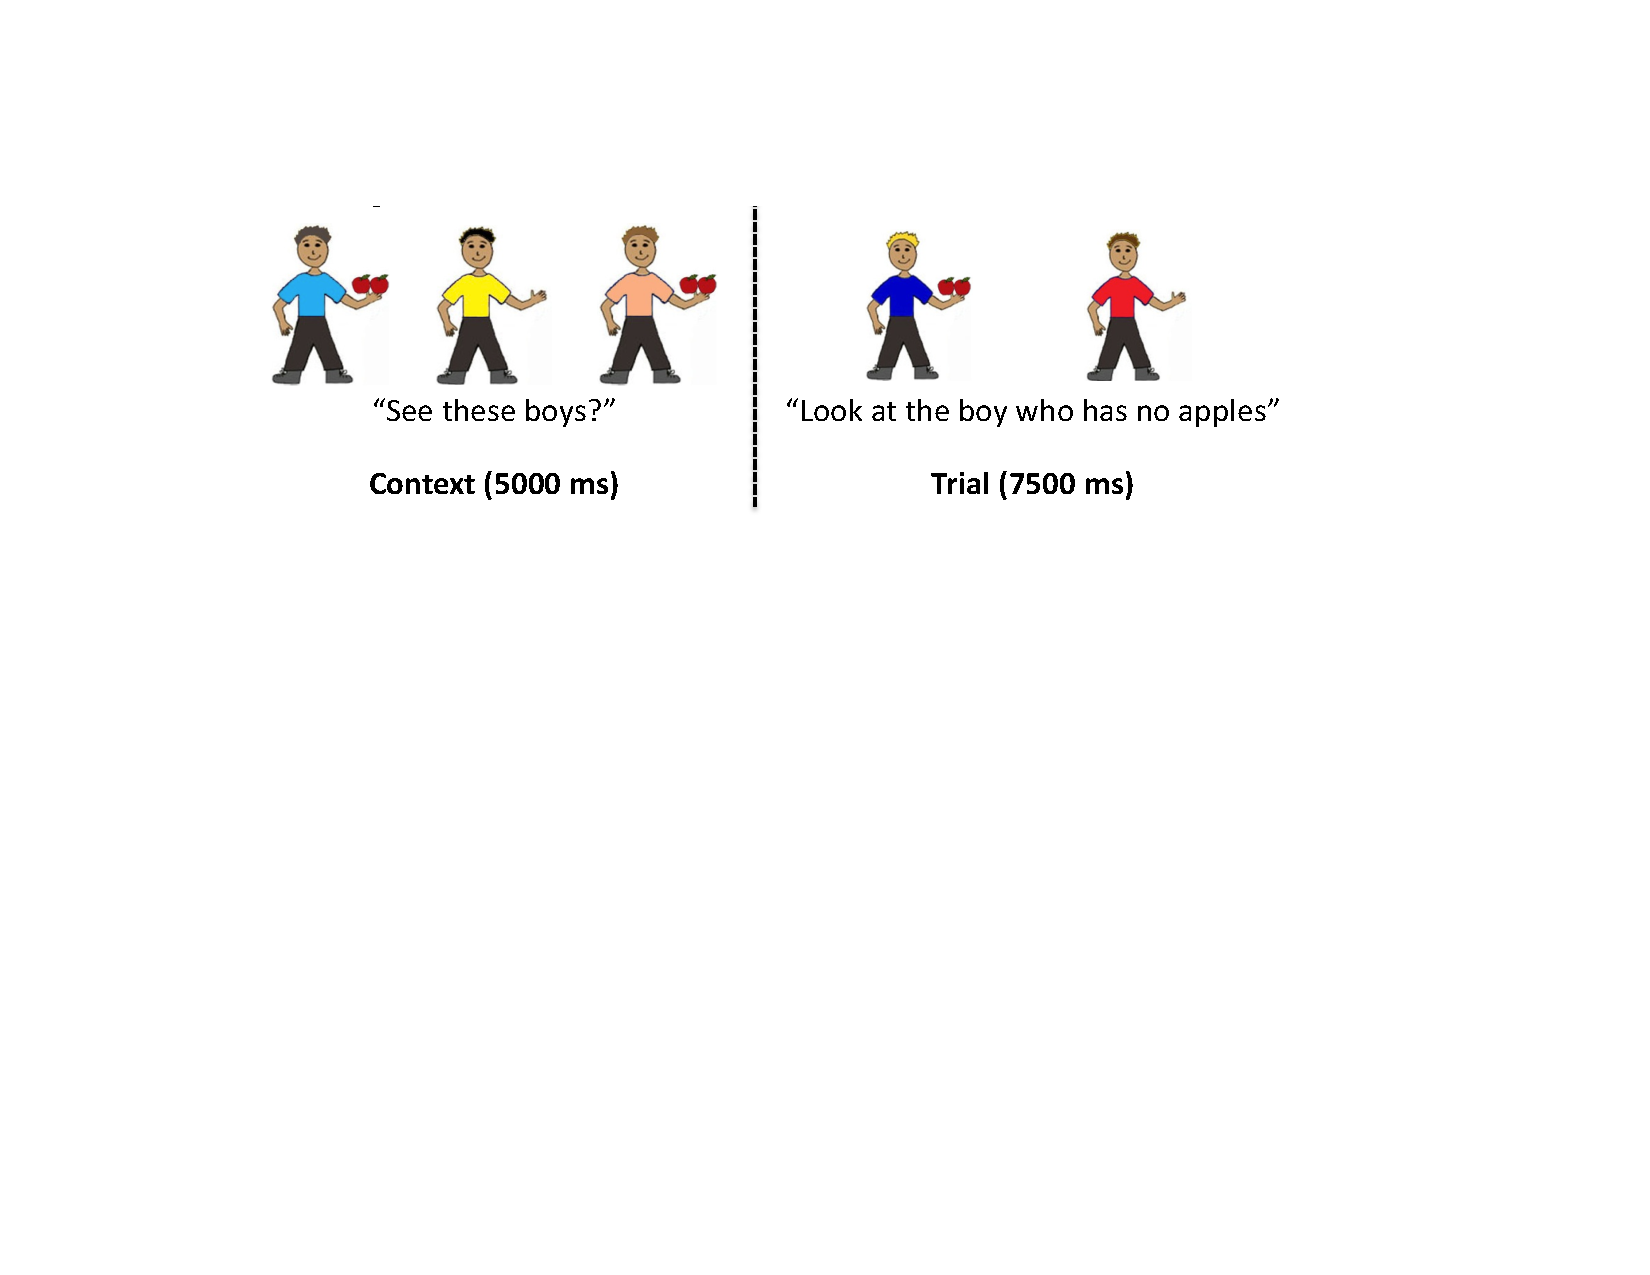
\includegraphics[width=5in]{trialfigure_nothing.pdf}
\caption{\label{fig:e1stim} An example of context and negative test trial slides from Experiment 1. }
\end{center} 
\end{figure}

We created 16 items, each presented as an individual trial, such that each item was only seen in a single trial.  Items consisted of boys or girls either holding nothing or holding a pair of objects (e.g. two apples).  Each trial was matched with a positive or a negative sentence.  Sentences were of the form ``Look at the boy who has/has no apples.''  Each trial contained three parts: a context, a test trial, and feedback (see Figure \ref{fig:e1stim}):

\emph{Context.}  The context consisted of three characters, two holding two target items each, and the other character holding nothing.  A pre-recorded voice said e.g. ``See these boys?''  Each context lasted 5 seconds.  

\emph{Test trial.}  Each trial consisted of two new characters, one holding two target items and one holding nothing.  Positioning of the target character (i.e. the correct referent) as well as the positioning of the character holding the items was counterbalanced across trials.  The images were presented in silence for two seconds, after which a pre-recorded voice said a positive or a negative sentence (e.g. ``Look at the boy with/with no apples''), followed by an additional tag sentence (e.g. ``Can you find him?''). Each trial lasted 7.5 seconds. Positive and negative sentences were constructed using the same base audio (with a separate base sentence created for each gender, i.e. ``look at the boy who has'' or ``look at the girl who has'', to maintain a natural quality) with the positive and negative target items (e.g. ``apples'' / ``no apples'') spliced in using Audacity software.  Sentence prosody was constructed such that emphasis was placed on the final noun (e.g. ``apples'') in positive sentences and the word ``no'' in negative sentences.  Different items were used in each trial: carrots, cookies, cakes, spoons, buckets, oranges, lollipops, cars, kites, bananas, fish, balloons, apples, balls, ice cream, or flowers.

\emph{Feedback.}  Elmo (an animated red puppet) appeared next to the named character, accompanied by a chiming noise. This phase of each trial lasted 1.5 seconds.  

The experiment was presented in the form of a short video.  The video began with an Elmo video clip, during which any necessary adjustments to the eye-tracker were made.  This clip was followed by a 2-point calibration and a 4-point validation of the calibration points; deviation from the validation points was examined by the experimenter and the calibration sequence was rerun if deviation was excessive.  After calibration, children were introduced to Elmo and told that ``Today, Elmo is going to visit some of his friends.  Do you want to meet Elmo's friends?  Let's go!''  This opening sequence was created to give the video a more narrative framing, and to motivate children to look to the target characters during the test trials.  

Following this introduction, children saw three gaze-contingent practice trials, designed so that the video would not advance until the child looked at the target item. Practice trials involved only the trial and feedback sections, with no context slide.  The first practice item had only one character, while the next two practice items had two characters (congruent with the test trials).  

The rest of the video consisted of 16 trials, as well as 6 filler pictures of Elmo and 4 Elmo video clips.  Filler videos were advanced by the experimenter after a variable length of time depending on the child's attentiveness, making the total experiment length slightly different for each child. In general the video lasted 7 minutes.  Two versions of the test video were created, such that trial types were counterbalanced and trial order was pseudo-randomized across the two versions. 

\subsubsection{Procedure}

Parents and children were recruited on the floor of the CDM and were led to a small nearby research room.  Children sat in a booster seat approximately 60 cm from the monitor of an SMI RED 120 Hz corneal reflection eye-tracker mounted on an adjustable arm.  A small subset of children  (less than 10\%) sat on a parent's lap, depending on the child's age and level of comfort.  Parents were asked to look away from the screen during calibration, to confirm that the child's eyes were being tracked.  

\subsubsection{Eye-tracking analysis}

All data were exported from the SMI format to simple text files and processed using the R data analysis language. Data from blinks and other cases where track was lost were treated as missing and excluded from further analysis. Each trial was synchronized to the point of disambiguation, which was coded individually for each audio stimulus. The point of disambiguation for both positive and negative trials was defined as the onset of the target noun (e.g. ``apples'').  Although it is possible in this experiment that participants could infer that ``no'' refers to the boy with nothing, the target noun is required to confirm which character is the correct referent. Looks were coded as being on the correct target if they fell on the corresponding side of the screen (excluding a  400 pixel zone in the middle of the two targets).  

\subsection{Results and Discussion}

\begin{figure}
\begin{center} 
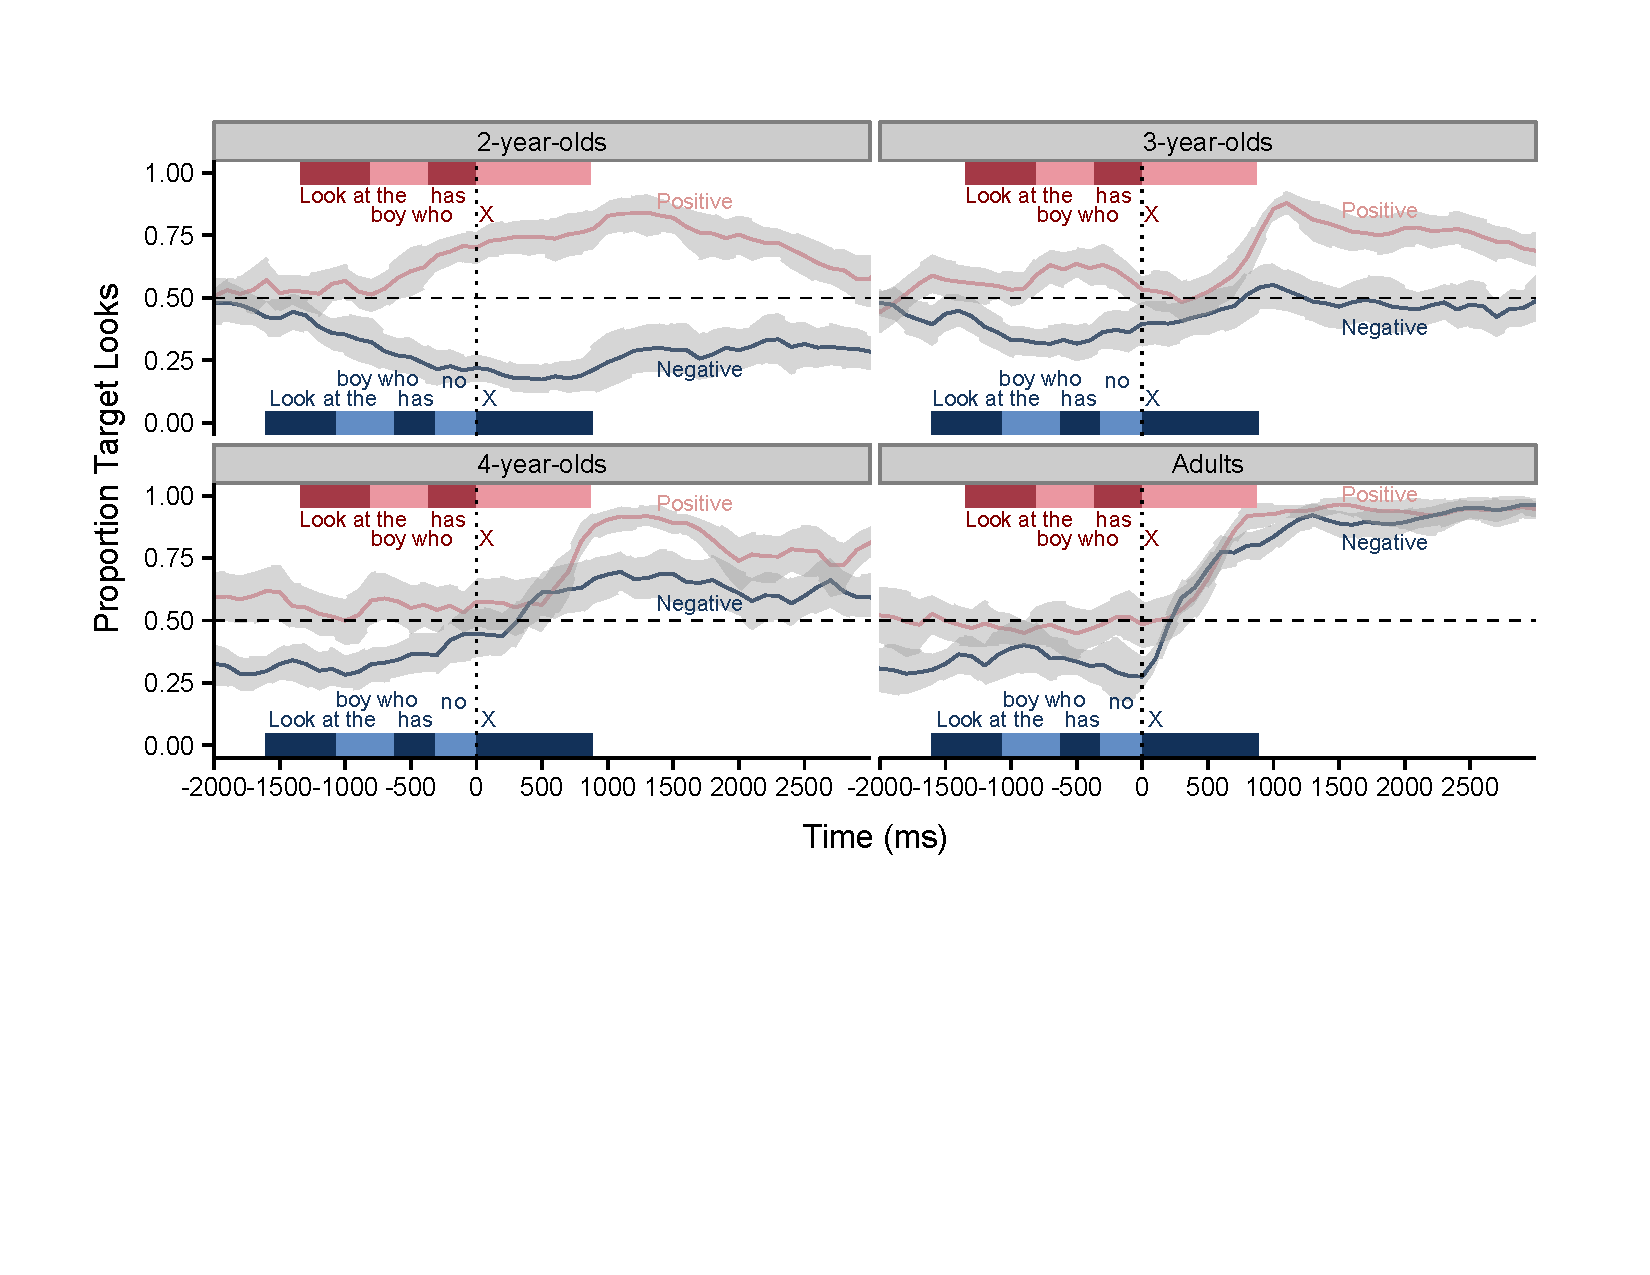
\includegraphics[width=6in]{simpleplots_nothing.pdf}
\caption{\label{fig:e1simple} Target preference plots for Experiment 1. Each panel shows the proportion of participants in a single age group (two-, three-, and four-year-olds and adults) who looked at the target picture for each trial type across time. Positive trials are shown in light pink and negative trials are shown in dark blue.  The vertical dotted line shows the onset of the final noun in each sentence. Average timings for individual words in positive and negative items are pictured at the top and bottom of each plot, respectively. The horizontal dashed line shows chance responding. Shaded regions show 95\% confidence intervals across participants.}
\end{center} 
\end{figure}

The majority of children in all age groups and conditions responded correctly to positive sentences, but there were substantial differences in accuracy on negative sentences across age groups. Figure \ref{fig:e1simple} shows the proportion of children who looked to the target picture over the course of a trial. Two-year-olds showed essentially no comprehension of negation in this paradigm, with children continuing to look away from the target picture throughout the duration of the trial, matching ``no apples'' to the picture of the boy \emph{with} apples.  Three-year-olds looked more at the target than did two-year-olds, but on average only 50\% were able to orient correctly to the target of negative sentences.  Only four-year-olds showed robust comprehension of negation, with 70\% of children looking correctly to the target of negative sentences by around a second after the onset of the final noun.  

Previous work with adults has shown delayed comprehension of negative sentences compared to positive sentences \cite{hclark1972, just1971, just1976, carpenter1975}.  On our task, however, adults appeared to show comparable performance on both positive and negative sentences.  Although adults showed a slight preference for the character with target items early in the trial (discussed below), they actually appear to shift their gaze to the target of negative sentences faster than they shift their gaze to the target of positive sentences (as indicated by the sharper change in slope at the disambiguating noun).  In fact, given that it takes 150-200 ms for adults to plan a saccade \cite{allopenna1998, rayner1998}, adults appear to be identifying the target of negative sentences as soon as they hear the word ``no.''  Unlike in previous studies of adults' negation processing, in our stimuli there is an obvious referent for the negation (e.g. the character with nothing).  It is possible that adults are making a prediction about which character is the referent of a negative sentence, even before they hear the disambiguating noun.   

Two- and three-year-olds' difficulty in responding to negative sentences is surprising, given that children at this age are robustly producing nonexistence negation using ``no'' \cite{bloom1970, pea1980}.  Why is it, then, that these children seem to be struggling to comprehend such sentences?  Onset-contingent plots can provide us with a more detailed way of looking at children's gaze behavior, and give us insight into how children are processing these sentences over the course of the trial.  These plots split trials based on whether the child was looking at the target or the distractor at the onset of the noun, and plot the proportion of children who shift their gaze to the opposite item.  In successful comprehension, children who are initially looking at the distractor should show rapidly increasing shifts to the target, whereas children who are initially looking at the target should continue to look at the target \cite{fernald2008}.  

\begin{figure}
\begin{center} 
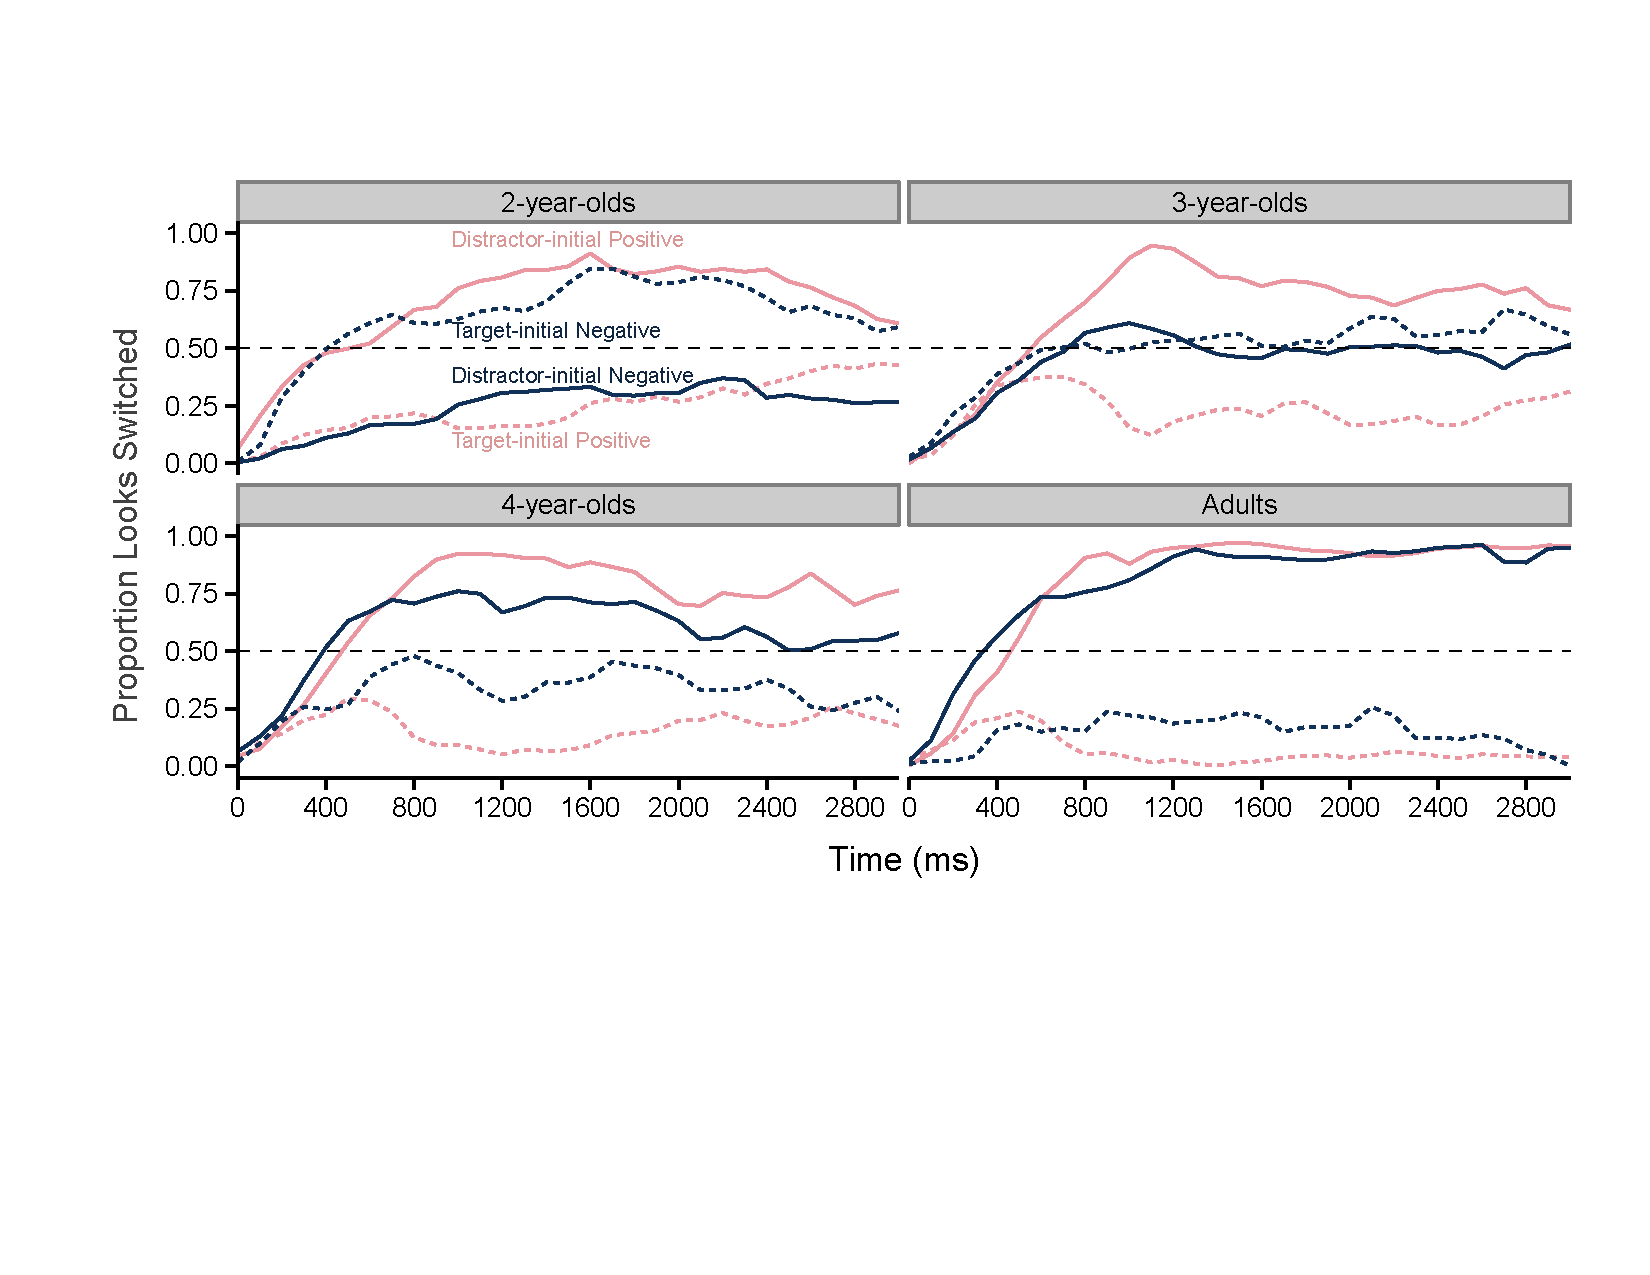
\includegraphics[width=6in]{OC_nothing.pdf}
\caption{\label{fig:e1split} Onset-contingent plots for Experiment 1. Each panel shows the looking behavior for participants in a single age group, beginning at the point of disambiguation (the noun onset). For each trial type, fixations are split by whether participants are looking at the target or the distractor at the point of disambiguation. Positive trials are shown in light pink and negative trials are shown in dark blue. For ``target-initial'' trials (dotted lines), looks to the distractor are plotted; correct responding is shown by continuing to look at the target. For ``distractor-initial'' trials (solid lines), looks to the target are plotted; correct responding is shown by shifting to the target. The horizontal dashed line shows chance.}
\end{center} 
\end{figure}

Onset-contingent plots for our data are shown in Figure \ref{fig:e1split}. Responses to the positive sentences are typical for such plots, but responses to the negative sentences deviate substantially from the expected pattern.  Two-year-olds actually showed the reverse pattern: If they were looking at the target picture, they oriented away, and if they were on the distractor, they stayed.  This suggests that two-year-olds were actually treating the negative sentences like positive sentences.  The onset-contingent plot of the three-year-olds' gaze data suggests general confusion; regardless of whether they started on the target or distractor picture, their looks to the target picture remained at chance.  Only four-year-olds showed the expected pattern, switching away from the distractor picture and staying on the target picture, though not as robustly as adults, who responded to negative sentences in the same way that they responded to positive sentences.  

% latex table generated in R 2.15.3 by xtable 1.7-1 package
% Tue Jun 18 10:02:29 2013
\begin{table}[ht]
\caption{\label{tab:e1model}Coefficient estimates from mixed-effects models predicting proportion of looks to target 300-2300 ms after noun onset (Experiment 1). }
\begin{center}
\small\addtolength{\tabcolsep}{-5pt}
\begin{tabular}{rrrr}
  \hline
 & Coefficient  & Std. Err. & $t$ value \\ 
  \hline
Intercept & 0.78 & 0.03 & 27.81 \\ 
  Age (Three-year-olds) & -.06 & 0.04 & -1.5 \\ 
  Age (Four-year-olds) & 0.00 & 0.04 & -.086 \\ 
  Age (Adults) & 0.09 & 0.04 & 2.28 \\ 
  Sentence (Negative) & -0.54 & 0.04 & -12.55  \\ 
  Age (Three-year-olds) $\times$ Sentence (Negative) & 0.28 & 0.06 & 4.94 \\ 
  Age (Four-year-olds) $\times$ Sentence (Negative) & 0.41 & 0.06 & 6.69 \\ 
  Age (Adults) $\times$ Sentence (Negative) & 0.49 & 0.07 & 7.42  \\ 
   \hline
\end{tabular}
\end{center}
\end{table}

To varying degrees, all four participant groups showed a baseline preference to look at the character who had something (rather than the target with nothing). Because our experimental design balanced positive and negative trials, this preference did not emerge from a learned expectation that one character type would be referred to more often. Instead, it likely came out of the fact that the character with something was more salient (whether visually or conceptually) and that---perhaps because of this greater salience---the same character was also \emph{a priori} more likely to be talked about \cite{frank2012}. Onset contingent plots also provide a method to control for baseline differences, at least partially \cite<but cf.>{grodner2010}.

\begin{figure}
\begin{center} 
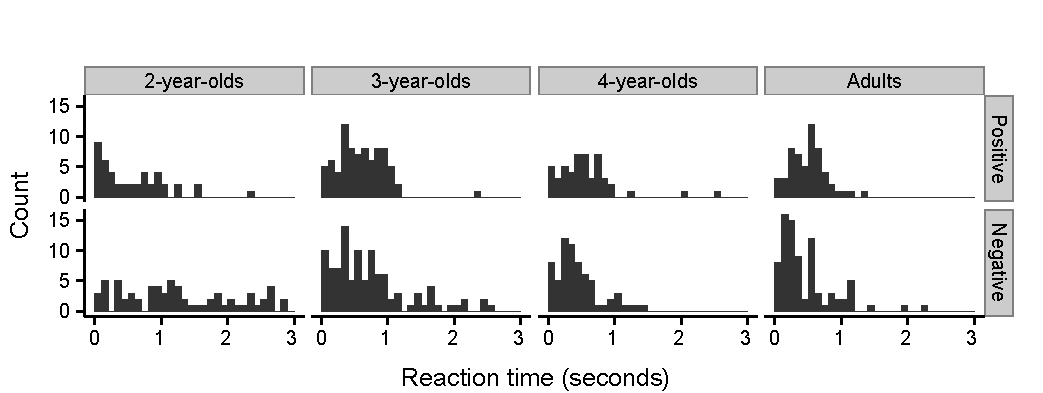
\includegraphics[width=6in]{RTs_nothing.pdf}
\caption{\label{fig:e1rt} Histograms of reaction times (time to first look to target) in response to individual distractor-initial trials in Experiment 1.  Panels from left to right show responses for participants in a single age group.  Top panels show responses to positive sentences, and bottom panels show responses to negative sentences.}
\end{center} 
\end{figure}

In addition to examining accuracies, we computed reaction times for distractor-initial trials, measuring the time to the first shift to the target picture after hearing the onset of the target noun \cite{fernald2008}.  Figure \ref{fig:e1rt} shows a histogram of participants' reaction times in response to individual trials.  Typically, participants' reaction times to shift to the target picture following a disambiguating word are normally distributed,  while times to shift to the distractor picture are uniformly distributed \cite{fernald2008}.  This pattern is interpreted as suggesting that shifts to the target are planned in response to the disambiguating noun, and shifts to the distractor reflect random shifts between the two objects.  

In our data, we examined reaction times for shifts to the target only. Three-year-olds, four-year-olds, and adults all showed normally distributed times to shift to the target of both positive and negative sentences. Thus, although three-year-olds only spent about 50\% of the time fixating on the correct picture on negative trials, evidence from their reaction times suggests that they nevertheless might have been making intentional shifts to the target in response to negation.  In contrast, two-year-olds shifts' to the target picture were uniformly distributed.  These shifts tended to occur faster for positive sentences than negative sentences, but in both cases these shifts appeared more uniform and less clearly yoked to the presence of the word ``no''.  This pattern of uniform responding is congruent with the accuracy data in Figure \ref{fig:e1split}, and suggests that two-year-olds were looking primarily to the positive target punctuated by occasional random switches to the negative target.  

To examine the reliability of our findings, we fit a linear mixed-effects model to dwell times on the target pictures. We analyzed the interaction between sentence type and age group on each participant's proportion looking to the target between 300 and 2300 ms following the onset of the noun for each trial.  The onset of this window was set at 300 ms to give children time to process the auditory information and plan an eye movement \cite{fernald2008, haith1993}, and the offset at 2300 ms occurred before before children saw any feedback about the correct referent of the sentence.   Coefficients for this model are shown in Table \ref{tab:e1model}.\footnote{Because of the robustness of the patterns we observed, for simplicity and interpretability we fit a linear model to proportions of looking within a target window rather than attempting to fit a series of logistic functions for individual time points. All mixed-effects models were fit using the lme4 package in R version 2.15.2.  The model specification was as follows: \texttt{on.target $\sim$ age~$\times$~sentence + (sentence~\textbar~subject) +  (age~\textbar~item)}. Data and analysis code can be found at \texttt{http://github.com/anordmey/Negtracker}.  Significance was calculated using the standard normal approximation to the $t$ distribution \cite{barr2013}.} Results of this model indicate a highly significant effect of sentence type, with significantly fewer children looking to the target picture in response to negative sentences compared to positive sentences ($\beta= -.54$, $p< .001$).   There were significant interactions between age group and sentence type for three-year-olds ($\beta = .28$, $p< .001$), four-year-olds ($\beta = .41$, $p< .001$), and adults ($\beta = .49$, $p< .001$), indicating that the increase in accuracy across development is driven primarily by improved comprehension of negative sentences.  

We conducted post-test analyses to analyze the effects of sentence type in each age group separately.  A model fit only to the data within each age group showed a significant difference in responses to positive and negative sentences for two-year-olds ($\beta = -.53$, $p< .001$), three-year-olds ($\beta = -.26$, $p< .001$), and four-year-olds ($\beta = -.14$, $p< .001$), with all children significantly less likely to look at the target of negative sentences compared to positive sentences.\footnote{The model specification for each age group was \texttt{on.target $\sim$ sentence + (sentence~\textbar~subject) +  (sentence~\textbar~item)}.}  Only adults showed similar responses to both positive and negative sentences, with no significant difference between the two sentence types ($\beta = -.05$, $p=.11$).  

Although four-year-olds performed significantly worse on negative sentences than positive sentences, a one-sample t-test of their responses to negative sentences showed that four-year-olds were significantly above chance (.5) at looking to the target of negative sentences ($t(23) = 4.14$, $p< .001$), as were adults ($t(15) = 13.9$, $p< .001$).  Three-year-olds responses to negative sentences were no different from chance ($t(30) = -.77$, $p=.46$), and two-year-olds were below chance ($t(23) = -7.12$, $p< .001$).  As discussed above, the difference in salience between the two pictures suggests that this may be a conservative test of comprehension.  The onset-contingent plots shown in Figure \ref{fig:e1split} and the distribution of reaction times seen in Figure \ref{fig:e1rt} suggest that while two-year-olds are looking almost entirely to the positive target (regardless of the sentence they heard), three-year-olds are starting to show some comprehension of the negative element.   

Together, these results reveal an interesting developmental pattern. Two-year-olds seemed to disregard the negative element completely, treating the negative sentences as positive; three-year-olds showed slightly improved performance but were still at chance in their responses to negative sentences.  Only by age 4 were children able to look reliably towards the correct referent of the negative items.  One possible explanation for the poor performance of two- and three-year-old children is that our materials created a challenging context for nonexistence negation.  Typically, nonexistence negation is produced in contexts where a salient object has disappeared, or when an expected object or action has failed to occur.  In contrast, our context required children to orient \emph{away} from the more interesting picture, creating an inhibitory demand in their orienting responses.  Perhaps two- and three-year-olds remained at or below chance in part because they knew that they \emph{should} look to the target, but they had difficulty shifting their attention away from the more salient picture and maintaining their attention on the target.  On this account, children have the conceptual knowledge necessary to understand negation, but the context is challenging for children because it requires them to inhibit their desire to look at the more interesting picture. If this is the case, children should show increased comprehension of negation in contexts where the possible targets of negation are equally salient.

\section{Experiment 2}

Experiment 1 found that children up to age four struggled to identify the referent of a negative sentence when that sentence referred to ``nothing.''  Because nonexistence negation is one of the first types of negation that children produce, it seems unlikely that this difficulty was due to lack of conceptual understanding.  A more likely explanation is that negative sentences in Experiment 1 required children to look at the character holding nothing, who was considerably less interesting.  When young children in naturalistic settings produce nonexistence negation, they are typically referring to an object that has recently disappeared from the scene or expressing surprise that an object is not in its expected location.  In addition, orienting away from a more interesting stimulus may require a level of cognitive or inhibitory control that two- and three-year-olds are not capable of.  In Experiment 2, we modified our stimuli so that the target of the negative sentences is holding a comparably interesting item that does not match the target noun (e.g. a boy holding presents on ``apples'' trials).  

Although the linguistic form of the negation in Experiment 2 remains identical (``no apples''), the conceptual form or complexity of the negation may be increased by the addition of a positive distractor item. Referring to a ``boy who has no apples'' in a case where the boy has nothing is certainly using negation to point out nonexistence. Using the same phrase in a case where the boy has something else (instead of apples) requires extra specificity to the inference: The child cannot simply match ``no'' to nonexistence, she must match ``no apples'' to the nonexistence of apples in particular. If comprehending negation is difficult for young children in part because these conceptual subtleties are challenging, then children in Experiment 2 should continue to show limited comprehension, because the conceptual demands are if anything increased.  If, however, children's performance in Experiment 1 is due to the fact that the context increased the cognitive demands of negative sentences, then children should have less difficulty responding to negative sentences in Experiment 2.

\subsection{Methods}

\subsubsection{Participants}

As in Experiment 1, families visiting the CDM were invited to participate.  Eleven children were excluded whose parents indicated that they were exposed to English less than 75\% of the time.  Eighteen children were excluded for being outside the target age range (between two and five years old).  Four children were excluded due to technical problems during the calibration phase.  This resulted in a sample of 93 children, 29 two-year-olds (mean age = 2;5, range = 2;0--2;11, 12 female), 34 three-year-olds (mean age = 3;5, range = 3;0--3;11, 15 female), and 30 four-year-olds (mean age = 4;5, range = 4;0--4;11, 20 female).  In exchange for participation, children were given a sticker and a certificate.  

The same rejection criteria were used as in Experiment 1.  Three two-year-olds and 3 three-year-olds were rejected for participating in fewer than 8 trials.  A further 2 two-year-olds, 3 three-year-olds, and 5 four-year-olds were rejected due to loss of gaze data in more than 30\% of the experiment.  This procedure left a total of 77 participants whose data was analyzed; 24 two-year-olds, 28 three-year-olds, and 25 four-year-olds. A comparison group of 16 adult participants (Stanford undergraduates) also participated as volunteers or in exchange for course credit; none were excluded.

\subsubsection{Stimuli}

\begin{figure}
\begin{center} 
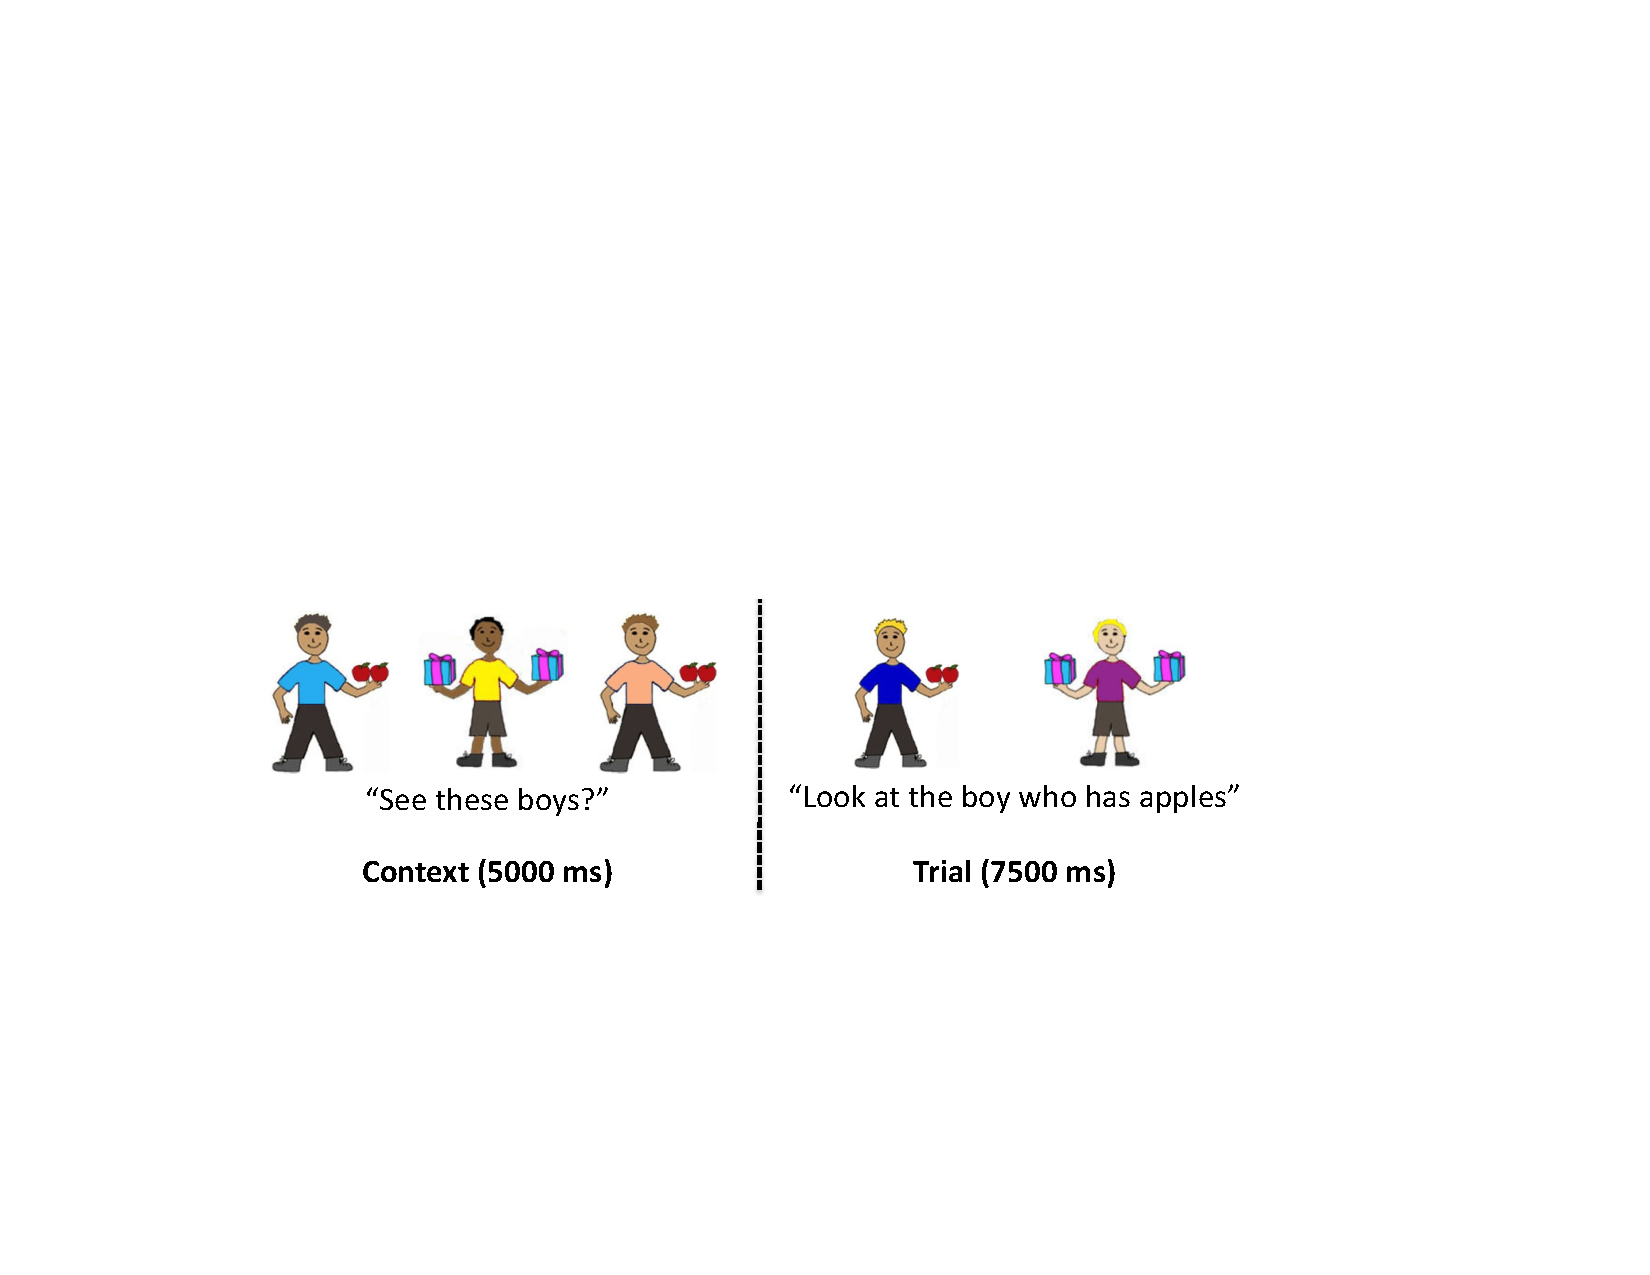
\includegraphics[width=5in]{trialfigure_something.pdf}
\caption{\label{fig:e2stim} An example of context and positive test trial slides from Experiment 2. }
\end{center} 
\end{figure}

As in Experiment 1, we created a total of 16 trials.  Items were identical to those presented in Experiment 1 except that in each context and test trial the boy or girl with nothing was replaced with a boy or girl holding different items (see Figure \ref{fig:e2stim}).  Thus, all characters in each trial were holding items, making all of the characters equally salient (given that items were counterbalanced).  Each trial was paired with a positive or negative sentence, identical to the sentences used in Experiment 1 (``Look at the boy who has/has no apples'').  As in Experiment 1, each trial contained three parts: a context, a test trial, and feedback.  The timing and presentation of the trials, and the construction of the video, was identical to Experiment 1.  

\subsubsection{Procedure}

The procedure was identical to the procedure used in Experiment 1.  

\subsubsection{Eye-tracking analysis}

All data analysis was identical to the previous experiment, except as noted below.

% Experiment 2 was designed to test children's comprehension of negative sentences that refer to alternatives.  Although this type of negation may be conceptually more complex, the fact that the two characters are equally salient reduces the inhibitory control required to respond correctly to the negative sentences.  If inhibitory control is responsible for children's poor performance in Experiment 1, we should see improved performance in this experiment.  

\subsection{Results and Discussion}

We begin by describing planned analyses of Experiment 2, which correspond to the analyses described above for Experiment 1. We then move on to a series of exploratory analyses of time-course effects that we discovered in our data.

\begin{figure}
\begin{center} 
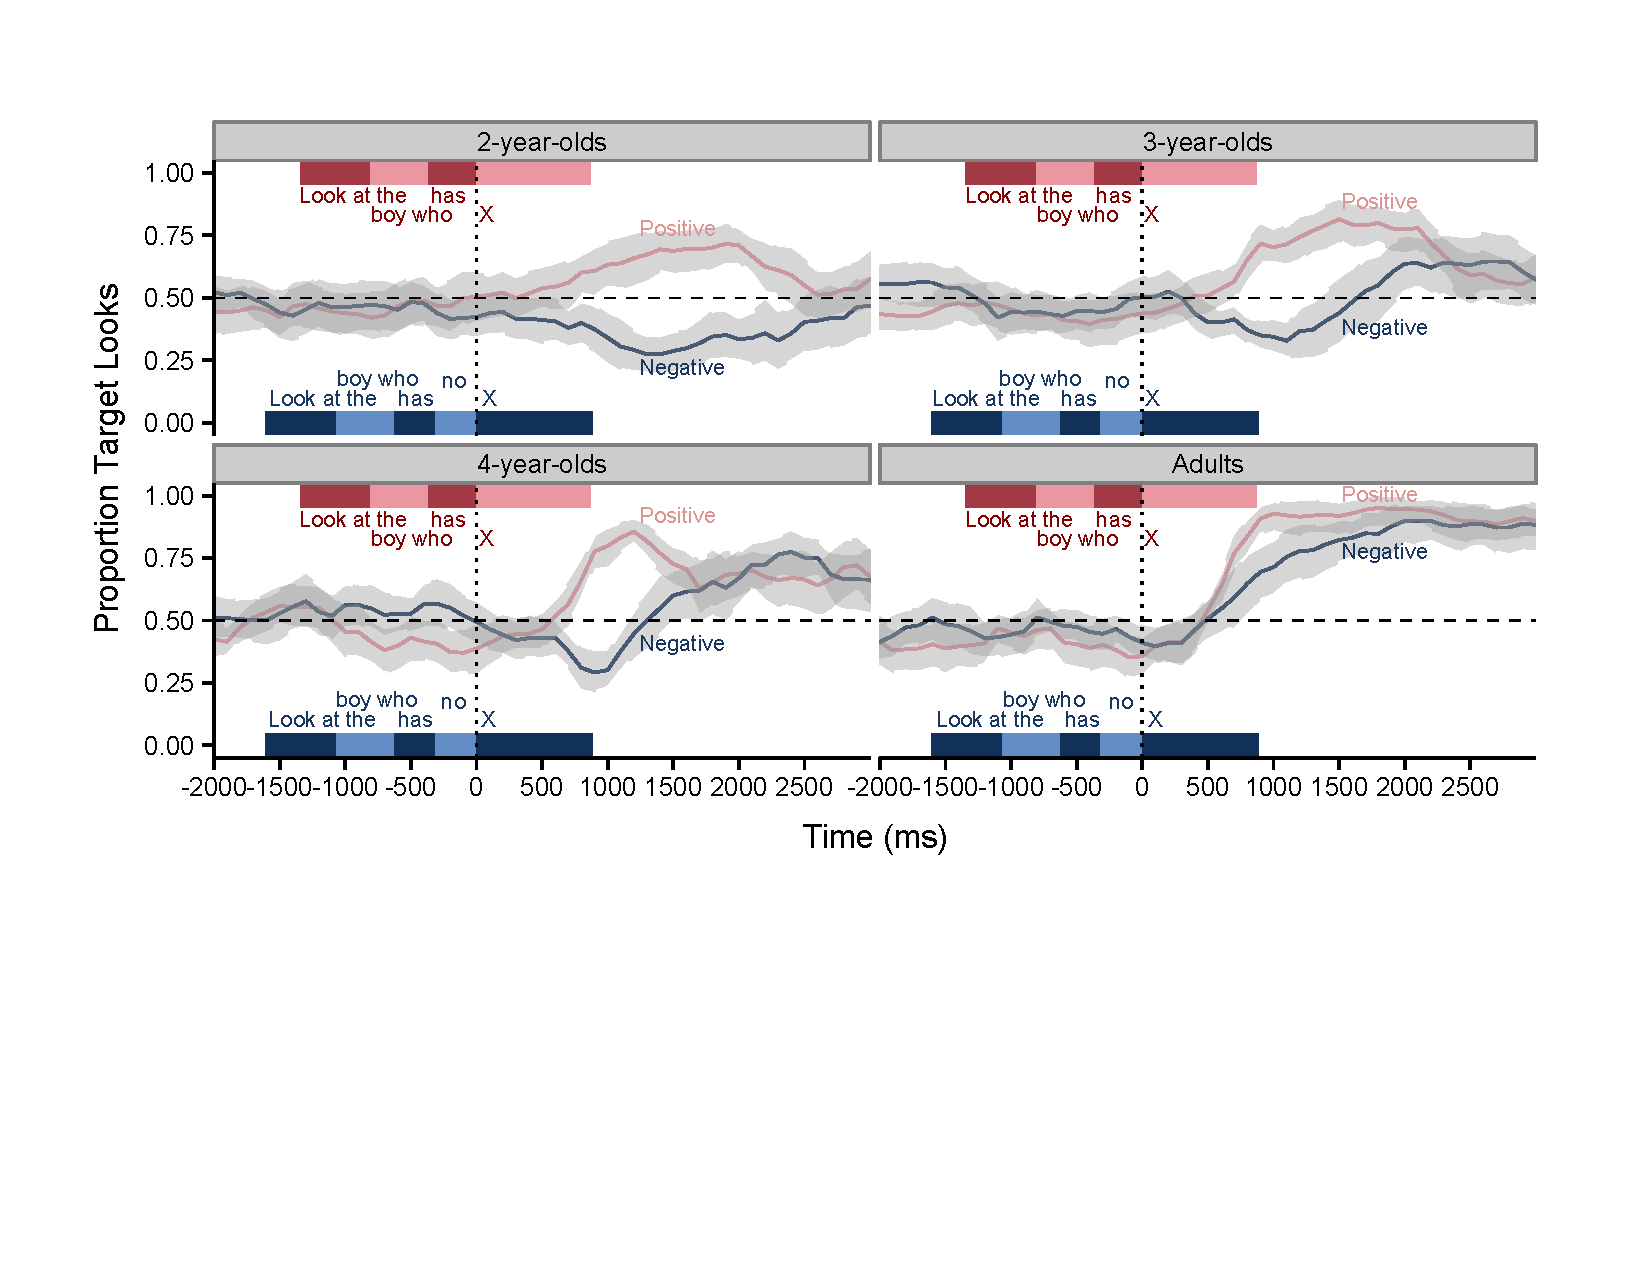
\includegraphics[width=6in]{simpleplots_something.pdf}
\caption{\label{fig:e2simple} Target preference plots for Experiment 2. Plotting conventions are the same as in Figure \ref{fig:e1simple}.}
\end{center} 
\end{figure}

\subsubsection{Planned Analyses}
Figure \ref{fig:e2simple} shows the proportion of children who looked to the target picture over the course of a trial.  As in Experiment 1, the majority of children in both age groups and conditions responded correctly to positive sentences.  Furthermore, two-year-olds continued to show no comprehension of the negative sentences, even though in this experiment both targets were equally salient.  Three-year-olds and four-year-olds showed a different pattern, however: Although both groups did eventually show some comprehension of negation, initially both groups looked \emph{away} from the target picture.  It was not until between 1200 and 1600ms that three- and four-year-olds began to look back towards the target picture in response to the negative sentences. Surprisingly, although this paradigm appeared to be easier for children, adults appeared somewhat slower to identify the referent of negative sentences than they were in Experiment 1.  

\begin{figure}[t]
\begin{center} 
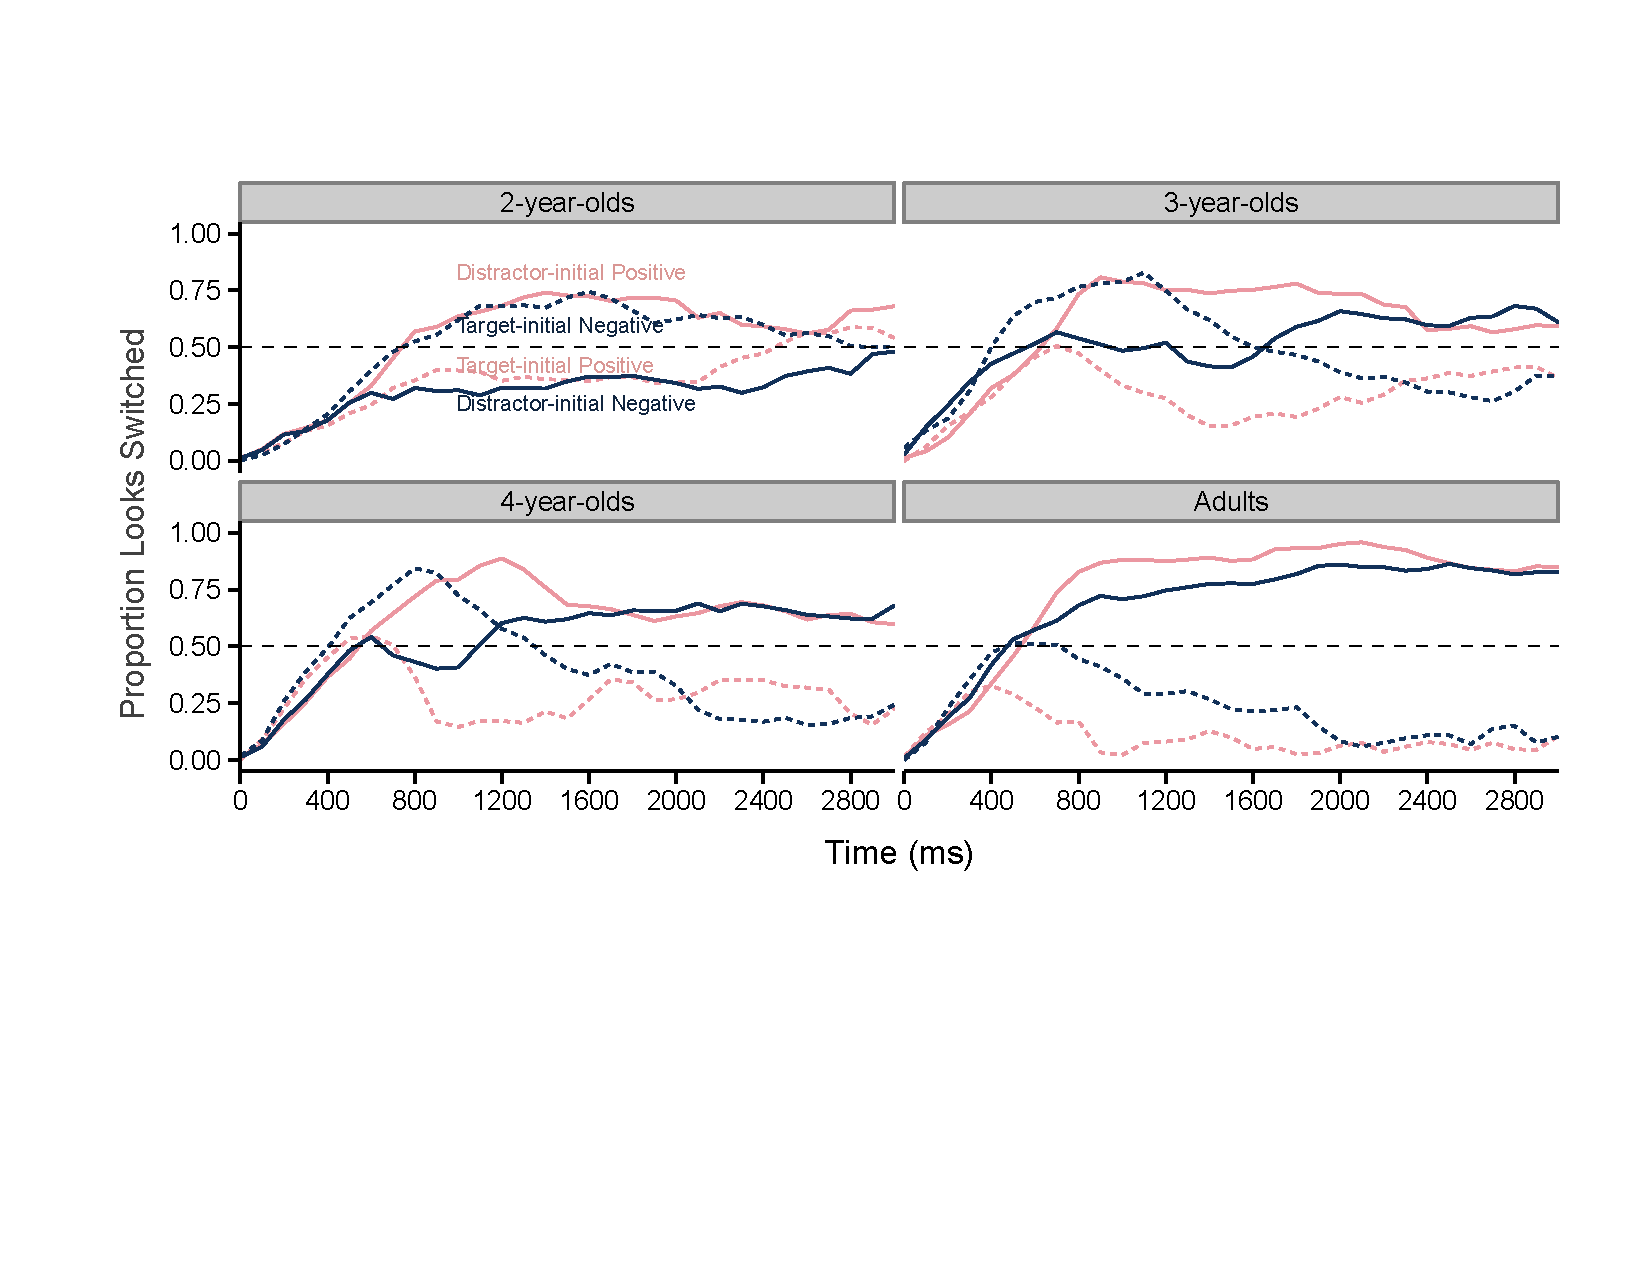
\includegraphics[width=6in]{OC_something.pdf}
\caption{\label{fig:e2split} Onset-contingent plots for Experiment 2. Plotting conventions are the same as in Figure \ref{fig:e1split}.}
\end{center} 
\end{figure}

The same developmental pattern can be seen even more clearly in onset-contingent plots (Figure \ref{fig:e2split}).  Three-year-olds who were looking at the distractor at the point of disambiguation continued to linger on the distractor until approximately 1600ms, at which point the majority of looks shifted to the target.  But three-year-olds who were looking at the target at noun onset shifted \emph{away} from the target, fixating the distractor until around 1600ms, when they looked back to the target.  This same pattern can be seen in the onset-contingent plots for the four-year-olds, except that for these older children this shift happened faster, around 1200ms following the onset of the noun.  Even adults showed a subtle tendency towards this pattern: Although adults who were originally fixating on the distractor were quick to shift to the target in response to both positive and negative sentences, adults fixating on the target when they heard a negative sentence showed a tendency to shift towards the distractor picture before looking back towards the target.  To summarize: In Experiment 2, all participants showed a tendency to look towards a named noun, even when that noun had been negated (e.g. looking towards the boy with apples even for a sentence ending with ``no apples''). 

% latex table generated in R 2.15.3 by xtable 1.7-1 package
% Tue Jun 18 10:03:46 2013
\begin{table}
\caption{\label{tab:e2model}Coefficient estimates from a mixed-effects model predicting proportion of looks to target in an early window (300-1300 ms after noun onset) and a late window (1300-2300 ms after noun onset) (Experiment 2).}
\begin{center}
\small\addtolength{\tabcolsep}{-5pt}
\begin{tabular}{rrrr}
  \hline
 & Coefficient  & Std. Err. & $t$ value \\ 
  \hline
Intercept & 0.59 & 0.03 & 20.18 \\ 
  Age (Three-year-olds) & 0.02 & 0.04 & .51 \\ 
  Age (Four-year-olds) & 0.06 & 0.04 & 1.56 \\ 
  Age (Adults) & 0.14 & 0.04 & 3.27 \\ 
  Sentence (Negative) & -0.22 & 0.04 & -4.95 \\ 
  Window (Late) & 0.11 & 0.04 & 2.74 \\ 
  Age (Three-year-olds)$\times$Sentence (Negative) & 0.00 & 0.06 & -0.06 \\ 
  Age (Four-year-olds)$\times$Sentence (Negative) & -0.04 & 0.06 & -0.79 \\ 
  Age (Adults)$\times$Sentence (Negative) & 0.10 & 0.06 & 1.75 \\ 
  Age (Three-year-olds)$\times$Period (Late) & 0.05 & 0.05 & 1.01 \\ 
  Age (Four-year-olds)$\times$Period (Late) & -0.05& 0.06 & -.86 \\ 
  Age (Adults)$\times$Period (Late) & 0.10 & 0.06 & 1.68 \\ 
  Sentence (Negative)$\times$Period (Late) & -0.16 & 0.05 & -3.12 \\ 
  Age (Three-year-olds)$\times$Sentence (Negative)$\times$Period (Late) & 0.13 & 0.07 & 1.85 \\ 
  Age (Four-year-olds)$\times$Sentence (Negative)$\times$Period (Late) & 0.36 & 0.07 & 4.95 \\ 
  Age (Adults)$\times$Sentence (Negative)$\times$Period (Late) & 0.19 & 0.08 & 2.58 \\ 
   \hline
\end{tabular}
\end{center}
\end{table}

\begin{figure}
\begin{center} 
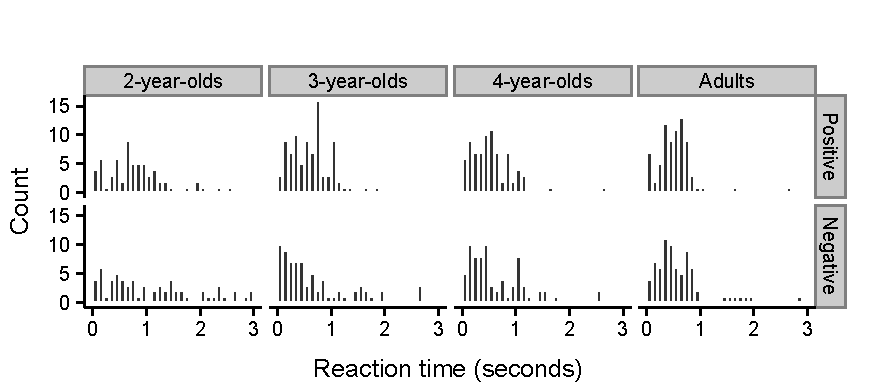
\includegraphics[width=6in]{RTs_something.pdf}
\caption{\label{fig:e2rt} Histograms of reaction times (time to first look to target) in response to individual distractor-initial trials in Experiment 2.  Panels from left to right show responses for participants in a single age group.  Top panels show responses to positive sentences, and bottom panels show responses to negative sentences.}
\end{center} 
\end{figure}

Figure \ref{fig:e2rt} shows a histogram of participants' reaction times in response to individual trials, again calculated as the time to the first shift to the target on distractor-initial trials \cite{fernald2008}. As in the previous experiment, three-year-olds, four-year-olds, and adult participants showed normally distributed times to shift to the target of both positive and negative sentences.  Unlike in the previous experiment, however, two-year-olds did show normally distributed responses to positive sentences; nevertheless, their responses to negative sentences still appeared to be uniformly distributed.  This analysis thus suggests that although two-year-olds' shifts to the target on positive trials were occurring in response to the target noun, their shifts to the target on negative trials likely indicate random shifts between the two characters.  

A linear mixed-effects model with the same structure as the model presented in Table 1 showed a similar but weaker pattern of effects as in Experiment 1. In examining the data, it appeared that the time-course effects were sufficient to obscure other trends. Rather than reporting this model, which averages across important signal, we instead report a series of exploratory analyses directly considering these time-course effects.

\subsubsection{Exploratory Analyses}

To capture the time-course effects we observed, we defined two temporal windows based on inspection of the data, bisecting the window of analysis explored in Experiment 1. The early window spanned from 300 to 1300 ms following the point of disambiguation, and the late window spanned from 1300 to 2300 ms following the point of disambiguation. We then fit a linear mixed effects model to test the interaction between sentence type, age group, and time window.\footnote{The model specification was \texttt{on.target $\sim$ age~$\times$~sentence~$\times$~window + (sentence + window~\textbar~subject) +  (sentence + age + window~\textbar~item)}.} Because our time windows were set post-hoc, we interpret statistical significance in this model with caution.  Results of this model suggest a significant effect of sentence type, with significantly fewer participants looking to the target picture in response to negative sentences compared to positive sentences ($\beta = -.22$, $p < .001$).   There were significant 3-way interactions between age group, sentence type, and time window for four-year-olds ($\beta = .37$, $p  < .001$) and adults  ($\beta = .19$, $p <.05$), and a marginally significant three-way interaction for three-year-olds ($\beta = .13$, $p =.06$), suggesting that in response to negative sentences, older children and adults showed an increase in looks to the target specifically in the later window of time. 

To compare the results of Experiment 1 to those of Experiment 2, we combined the data for both experiments and conducted an additional exploratory analysis, using a linear mixed-effects model to test the interactions between sentence type, age group, time window, and experiment on proportion looking to the target (full model shown in Appendix A).\footnote{The model specification was \texttt{on.target $\sim$ age~$\times$~sentence~$\times$~window~$\times$~experiment + (sentence + window~\textbar~subject) +  (sentence + age + window~\textbar~item)}.} The three-way interactions between age, sentence type, and experiment indicate that performance on negative sentences was \emph{lower} for three-year-olds ($\beta = - .39$, $p  < .001$), four-year-olds ($\beta = -.52$, $p <  .001$), and adults ($\beta = -.44$, $p  < .001$) on Experiment 2.  Examining Figure \ref{fig:e2simple}, this pattern appears to be due to children's looks to the incorrect picture in the initial period and adults' slower latency to target in response to negative sentences.  The delay in identifying the target leads to overall lower performance in response to negative sentences in Experiment 2.  In the 4-way interactions, however, which include the effect of time window, we now see \emph{increased} late performance on negative sentences for three-year-olds ($\beta = .34$, $p < .001$), four-year-olds ($\beta = .53$, $p < .001$), and adults ($\beta = .30$, $p <  .01$) in Experiment 2.  Thus, although target looking in Experiment 2 was lower than performance on Experiment 1 in the earlier window of time, in the later window of time performance increased such that three-year-olds now showed comprehension of negative sentences, and four-year-olds showed improved accuracy.  

In order to further explore the different processing patterns seen in Experiment 1 and Experiment 2, we fit separate models to the data for three- and four-year-olds to test the effects of sentence type, time window, and experiment on proportion looking to target.\footnote{The model specification for each age group was \texttt{on.target $\sim$ sentence~$\times$~window~$\times$~experiment + (sentence + window~\textbar~subject) +  (sentence + window~\textbar~item)}.} The model fit only to the three-year-olds' data failed to show a significant three-way interaction between sentence type, time window, and experiment  ($\beta = .09$, $p < .2$).  In contrast, this three-way interaction was significant for four-year-olds, indicating that their responses were significantly improved in response to negative sentences in the late window of Experiment 2  ($\beta = -.03$, $p < .38$).  Examination of Figures \ref{fig:e2split} and \ref{fig:e2simple} suggests that the bisection of the time window at 1300 ms may not accurately capture the gaze pattern displayed by three-year-olds, because these children do not appear to shift to the target of negative sentences until approximately 1600ms.  An additional post-hoc analysis of the three-year-old data using windows from 600-1600ms and 1600-2600 ms found a significant 3-way interaction between sentence type, time window, and experiment ($\beta = .22$, $p < .01$).  The results of these models together suggest that the gaze patterns reflected in Figures \ref{fig:e2split} and \ref{fig:e2simple} are due to significant differences in how three- and four-year-olds processed negative sentences in these two contexts.  

Although adults in Experiment 2 appeared slightly slower to process negations than they were in Experiment 1, a model fit only to the adult data did not find a significant interaction between sentence type, time window, and experiment ($\beta = -.05$, $p = .45$).  This model of only the adult data also failed to show a significant main effect of negation ($\beta = -.04$, $p = .3$).  There was a marginal interaction between sentence type and experiment ($\beta = -.03$, $p = .09$), suggesting that adults' slower performance on Experiment 2 may have been driven primarily by their performance on negative sentences.  Overall, however, these results suggest that the effect of negation on adults' performance was slight, at least in this relatively simple and repetitive paradigm.  

\subsubsection{Summary of Experiment 2 Results}
In the contexts of Experiment 2, three- and four-year-old children initially oriented towards the picture that matched the named noun (e.g. ``apples''), even when the noun was negated.  There are a number of possible explanations for this pattern.  One possibility is that this context is pragmatically infelicitous.  In the example shown in Figure 4, children may have expected to hear either ``apples'' or ``presents'' to describe the boys; ``no apples'' is an odd choice because it is a more costly utterance (requiring an additional word) and does not specify what the target character \emph{is} holding.  However, it is not clear why this would cause children to look \emph{away} from the target character as opposed to simply taking longer to orient to the correct character.  Another explanation is that it took children longer to fully integrate the negative element (``no'') with the referent (``apples'').  This could explain the tendency to shift away from the target upon hearing the disambiguating noun in Experiment 2, as well as very young children's difficulty with our task in both conditions (e.g. two-year-olds may not have been able to integrate the negative element in the time provided).  Finally, it is possible that when children are presented with two equally likely alternatives, identifying the referent of negation requires ruling out the named object.  That is, when children heard the phrase ``no apples'', they may have first tried to find the boy \emph{with} apples in order to rule him out as a possible target.  This would explain why children in all age groups systematically oriented away from the target character even if they were fixating on the target when they heard the disambiguating noun.  Further work is needed to clarify why children in Experiment 2 displayed this initial tendency to look away from the referent of negative sentences.  

Despite the fact that children heard the exact same sentences in Experiments 1 and 2, their comprehension appeared different in these different contexts.  Two-year-olds struggled to maintain looks to the target picture of negative sentences in both contexts, even though there was no baseline preference for either item in Experiment 2.  Three-year-olds failed to show robust comprehension of negation in a context where the negative sentences referred to the absence of an object (Experiment 1), but showed improved comprehension late in the trial when negative sentences referred to an alternative object (Experiment 2).  Four-year-olds showed comprehension of negation in both experiments, but like three-year-olds, their comprehension was delayed in Experiment 2.  These results suggest that different contexts of negation---in these experiments either a target with an absent feature, or a target with an alternative feature---led children to process these sentences in very different ways.  

\section{General Discussion}

Negative utterances emerge very early in children's productive speech, expressing a wide variety of concepts such as nonexistence, refusal, prohibition, and denial.  Despite this early emergence, and the importance of negation in human language and reasoning, we still know very little about how children process and comprehend negative utterances.  

We conducted a study of children's comprehension of negation in which negative sentences referred either to an absent item (Experiment 1) or an alternative item (Experiment 2).   We proposed several factors that might influence children's acquisition of negation, including linguistic factors (which were held constant in these experiments), conceptual factors, and pragmatic factors.  Experiment 1 tested a type of simple nonexistence that emerges early in children's production \cite{pea1980}.  It is possible that previous tests of children's negation comprehension have failed because these experiments have focused on denial negation, which might be conceptually more complex.  In Experiment 2, the context of the negative sentences required children to go beyond simply matching ``no'' to nonexistence in general and identify a specific nonexistence (``no apples''), making this type of negation more like the denial negation that has been tested in most previous studies of negative sentence comprehension.  If conceptual factors are of primary importance in children's comprehension of negation, Experiment 2 should have been more difficult for younger children.  Instead, children showed a different pattern of comprehension in Experiment 2, with three- and four-year-olds looking away from the target object early in the trial, but showing improved comprehension several seconds later.  These results suggest that pragmatic factors, rather than conceptual difficulty, may play a primary role in children's comprehension of negation.

If pragmatic factors play a large role in the acquisition of negation, the hypothesis that follows is that children can use and understand many types of negation at an early age, but that their ability to do so is limited by the contexts in which these negations are salient.  That is, children's difficulty in these experiments---particularly Experiment 1---maybe be due to the context of these experiments, rather than their conceptual or linguistic understanding of the word ``no.''  Although the context slides presented in this experiment have been shown to set up a strong expectation in adults (e.g. that boys have apples, \citeNP{nordmeyer2014}), it is possible that these contexts did not sufficiently change children's expectations, or that this expectation did not facilitate children's processing of the negative sentence.  Children in our experiments may have expected speakers to talk about the character with target items (Experiment 1), or to refer to characters by naming the target items (Experiment 2), leading them to spend more time fixating on the distractor after hearing a negative sentence.

Children's expressions of negation often occur in feeding situations, where a child has recently finished their food or drink (e.g. ``no juice'', Bloom 1970), or in situations where an object is not in its expected location or an expected action fails to occur.  In fact, in his investigation of children's early negative utterances, \citeA{pea1980} splits nonexistence into two categories, disappearance and unfulfilled expectations.  Both of these types of negation would occur in contexts where the absence of an item is highly salient, either because it has recently disappeared or an expectation has been violated.  Children may have an easier time comprehending negation in contexts where there is a strong expectation that an action will occur or an object will be present, or when the negated object was highly salient to the child.  Future work will explore how children's sensitivity to the pragmatics of negation influences their comprehension of negative sentences.

One way that children's difficulty with negation might manifest itself is through increased inhibitory demands in certain contexts.  In his investigation of children's early negative utterances, \citeA{pea1980} identified the development of self-prohibition as a critical step in children's acquisition of negation.  Although Pea was particularly interested in cases where a child succeeds in inhibiting their own actions after producing a self-prohibition, the opposite case is equally interesting in light of the results of the present studies.  Children who utter the word ``no'' while reaching towards a desired but forbidden object may understand the meaning of the word ``no,'' and understand that they are not supposed to touch what they are reaching for.  But in many cases these children still proceed with the prohibited action; although they understand the concept of prohibition, they do not have the inhibitory control necessary to stop their own actions. 

Following this line of reasoning, children's difficulty in Experiment 1 could be explained by the increased inhibitory demands imposed by the difference in salience between the two characters. Young children may have had difficulty looking away from the more interesting stimulus even if they understood the negative sentence. This account could explain why three-year-olds in Experiment 1 appeared to be performing at chance, but showed normally distributed reaction times in response to negative sentences: They understood the negation and were able to comprehend it appropriately (causing the RT distribution), but were nevertheless unable to inhibit shifts to the more salient distractor (causing the lower overall accuracy). It may have been easier for younger children to inhibit their shifting response in Experiment 2, when the correct alternative and the distractor were equally salient.  Naturalistic contexts likely alleviate inhibitory demands of this type; for example, a parent expressing prohibition might say the word ``no'' with fearful or angry vocal affect, providing children with a strong, additional cue to inhibit their action. By removing this sort of ecological cue, our paradigm arguably presented a more difficult case of comprehension than most that children encounter.  Adult participants (who typically have stronger capacities for inhibitory control than children under 5 years of age) responded quickly and accurately to negative sentences in Experiment 1, finding this task if anything slightly easier than Experiment 2.  Thus, although Experiment 2 may have been slightly more conceptually challenging, children's performance suggests that they had more difficulty with the cognitive demands that arose when negative sentences were presented within an insufficient pragmatic context.

Our findings suggest a possible synthesis of previous research on negation, encompassing both adults' comprehension and children's production.  Although adults' difficulty comprehending negation and children's early production may initially appear contradictory, the pragmatics of negation can help us resolve this paradox.  Just as adults' ability to process negative sentences is strongly influenced by the presence of a supportive context \cite<e.g.>{wason1965}, children in our experiments displayed a very different pattern of comprehension depending on the context in which the same sentence was presented.  Further exploration of the role of pragmatics in negative sentence processing and the specific contexts which make negation salient for children is essential to understanding the development of children's comprehension of negation.  


\bibliographystyle{apacite}
\bibliography{negtracker}

\newpage
% \appendix
\theappendix 


\section{Appendix A: Coefficients for Cross-Experiment Mixed-Effects Model}
\label{app:coef}

% latex table generated in R 2.15.3 by xtable 1.7-1 package
% Wed Jun 26 23:18:35 2013
\begin{table}
\label{tab:bothmodel}
\caption{Coefficient estimates from a mixed-effect model predicting proportion of looks to target in an early window (300-1300 ms after noun onset) and a late window (1300-2300 ms after noun onset), with Experiment as an additional factor.}

\begin{center}
\small\addtolength{\tabcolsep}{-5pt}
\begin{tabular}{rrrr}
  \hline
 & Coefficient  & Std. err & $t$ value \\ 
  \hline
Intercept & 0.78 & 0.03 & 25.00 \\ 
  Age (Three-year-olds) & -0.11 & 0.04 & -2.84 \\ 
  Age (Four-year-olds)&- 0.04 & 0.04 &  -.97\\ 
  Age (Adults) & 0.16 & 0.05 & .36 \\ 
  Sentence (Negative) & -0.58 & 0.05 & -12.17 \\ 
  Window (Late)  & -0.18 & 0.04 & -.48 \\ 
  Experiment (Exp. 2) & -0.20 & 0.04 & -4.95 \\ 
  Age (Three-year-olds)$\times$Sentence (Negative) & 0.38 & 0.06 & 6.40 \\ 
  Age (Four-year-olds)$\times$Sentence (Negative) & 0.47 & 0.06 & 7.41 \\ 
  Age (Adults)$\times$Sentence (Negative) & 0.54 & 0.07 & 8.02 \\ 
  Age (Three-year-olds)$\times$Window (Late)  & 0.12 & 0.05 & 2.42 \\ 
  Age (Four-year-olds)$\times$Window (Late) & 0.11 & 0.05 & 1.99 \\ 
  Age (Adults)$\times$Window (Late)  & 0.15 & 0.06 & 2.73 \\ 
  Sentence (Negative)$\times$Window (Late)  & 0.09 & 0.05 & 1.87 \\ 
  Age (Three-year-olds)$\times$Experiment (Exp. 2)  & 0.13 & 0.06 & 2.38 \\ 
  Age (Four-year-olds)$\times$Experiment (Exp. 2)  & 0.10 & 0.06 & 1.71 \\ 
  Age (Adults)$\times$Experiment (Exp. 2) & 0.15 & 0.06 & 1.99 \\ 
  Sentence (Negative)$\times$Experiment (Exp. 2)& 0.36 & 0.06 & 5.68 \\ 
  Window (Late)$\times$Experiment (Exp. 2)  & 0.13 & 0.05 & 2.37 \\ 
  Age (Three-year-olds)$\times$Sentence (Negative)$\times$Window (Late) & -0.22 & 0.07 & -3.24 \\ 
  Age (Four-year-olds)$\times$Sentence (Negative)$\times$Window (Late)  & -0.17 & 0.07 & -2.41 \\ 
  Age (Adults)$\times$Sentence (Negative)$\times$Window (Late)  & -0.11 & 0.07 & -1.46 \\ 
  Age (Three-year-olds)$\times$Sentence (Negative)$\times$Experiment (Exp. 2)  & -0.39 & 0.09 & -4.52 \\ 
  Age (Four-year-olds)$\times$Sentence (Negative)$\times$Experiment (Exp. 2)  & -0.52 & 0.09 & -5.77 \\ 
  Age (Adults)$\times$Sentence (Negative)$\times$Experiment (Exp. 2) & -0.44 & 0.10 & -4.57 \\ 
  Age (Three-year-olds)$\times$Window (Late)$\times$Experiment (Exp. 2)  & -0.06 & 0.07 & -.87 \\ 
  Age (Four-year-olds)$\times$Window (Late)$\times$Experiment (Exp. 2)  & -0.16 & 0.08 & -2.02 \\ 
  Age (Adults)$\times$Window (Late)$\times$Experiment (Exp. 2)  & -0.05 & 0.08 & -.68 \\ 
 Sentence (Negative)$\times$Window (Late)$\times$Experiment (Exp. 2)  & -0.25 & 0.07 & -3.59 \\ 
  Age (Three-year-olds)$\times$Sentence (Negative)$\times$Window (Late)$\times$Experiment (Exp. 2)  & 0.34 & 0.10 & 3.57 \\ 
  Age (Four-year-olds)$\times$Sentence (Negative)$\times$Window (Late)$\times$Experiment (Exp. 2)  & 0.53 & 0.10 & 5.26 \\ 
  Age (Adults)$\times$Sentence (Negative)$\times$Window (Late)$\times$Experiment (Exp. 2) & 0.30 & 0.10 & 2.89 \\ 
   \hline
\end{tabular}
\end{center}
\end{table}
\doublespacing

\end{document}


% the issues of inhibitory control that arose in our experiments may be reduced. Future work should therefore examine the contexts in which children are most likely to hear or produce negations.


% Although we made an attempt to situate our experimental negations in a context, these contexts were likely not as salient or as meaningful as the contexts naturally produced in an interaction with a parent or caregiver. 

% Our experiments examined nonexistence negation, in which the negative sentence refers to the absence of an object. This type of negation is one of the earliest to emerge in children's production \cite{pea1980, bloom1970}.  Nevertheless, we found that 2- and 3- year old children struggled to identify the referent of these sentences, and only by age 4 were children able to correctly orient to the target picture upon hearing a negative sentence in both experiments.  It seems unlikely that these results were due to children's failure to understand the concept of nonexistence, given that many children produce nonexistence negation by age 2. 



% A more likely explanation is that orienting to the target in these trials required greater inhibitory control because the target character is less interesting to children. This is an inherent part of nonexistence negation; by definition nonexistence refers to the absence of something.  It is likely that situations like this, where children are asked to identify a nonexistent referent alongside more salient alternatives, are more challenging than situations where a child describes her juice cup as having ``no more juice,'' where the nonexistence of juice is a salient feature.  

% In Experiment 2, we addressed these concerns by creating a new set of stimuli in which the negative sentence referred to a person with different objects.  Thus, when children heard ``Look at the boy with no apples'' they were being asked to look at the boy holding presents.  This can potentially construed as denial or truth-functional negation, because instead of simply identifying the absence of an object, children must determine which picture matches the truth of the sentence.  In this experiment, while two-year-olds continued to struggle to comprehend negative sentences, three-year-olds and four-year-olds now both were able to correctly identify the referent of negative sentences.  

% Although adults did not show the pattern that children displayed of initially orienting away from the target, they were slower to respond to negative sentences in Experiment 2 compared to Experiment 1.  Interestingly, this suggests that adults actually had more difficultly responding to negative sentences in Experiment 2 than in Experiment 1, unlike children, who showed comprehension at a younger age in Experiment 2.  As mentioned previously, it is possible that the negative utterances in Experiment 2 required more complex conceptual skills than the negation in Experiment 1.  While Experiment 1 only requires you to identify nonexistence, Experiment 2 requires you to evaluate the meaning of a denial negation and identify the picture for which that denial is true.  Perhaps this increased conceptual difficulty lead to slow response times even for adults, whereas for children, the greater inhibitory control required in Experiment 1 interfered with their ability to orient to the target even though the task was conceptually easy.  


% In two studies, we found that children continue to struggle to comprehend negative sentences in certain contexts up through age 4.  These results are surprising, in part because most children begin producing negation before age 2 \cite{pea1980}.  In particular, children's pervasive difficulty with processing nonexistence negation (Experiment 1) is unexpected because nonexistence is one of the first types of negation that children begin to produce.  This work demonstrates that conceptual difficulty is not the only aspect of negation that should be considered when evaluating how complex a negative sentence is for a child.  Depending on the context that a sentence is presented in, even conceptually simple negative sentences may require a great deal of inhibitory control to comprehend.  Children struggle to identify ``nothing,'' or to look away from a named object, and recognizing this difficulty is an important step in understanding children's acquisition of negation.  
